\documentclass[11pt]{article}

\usepackage[T1]{fontenc}
\usepackage{lmodern}
\usepackage{microtype}
\usepackage[margin=1in]{geometry}
\usepackage{amsmath,amssymb,amsthm,mathtools}
\usepackage{booktabs,longtable,array}
\usepackage{enumitem}
\usepackage{seqsplit}
\usepackage{xcolor}
\usepackage{listings}
\usepackage{tikz}
\usetikzlibrary{arrows.meta,positioning,fit,shapes.multipart}
\usepackage{fancyhdr}
\usepackage{hyperref}
\usepackage[nameinlink,noabbrev]{cleveref}

\hypersetup{
  colorlinks=true,
  linkcolor=blue!45!black,
  citecolor=blue!45!black,
  urlcolor=blue!55!black,
  pdftitle={Contender 11: Self-Height Diagonal Forest Closure of Kind-Polymorphic Reflection},
  pdfauthor={Research proposal for BusyLean}
}

\pagestyle{fancy}
\fancyhf{}
\lhead{BusyLean Contender 11}
\rhead{Self-height diagonal forest closure}
\cfoot{\thepage}
\setlength{\headheight}{14pt}

\definecolor{codebg}{RGB}{247,248,250}
\definecolor{codeframe}{RGB}{205,210,218}
\definecolor{codecomment}{RGB}{78,105,87}
\definecolor{codekeyword}{RGB}{38,69,126}
\lstdefinelanguage{Lean}{
  morekeywords={def,theorem,namespace,end,import,by,have,exact,show,match,with,fun,let,in,where,induction,generalizing,cases,unfold,change,open,obtain,refine,if,then,else},
  sensitive=true,
  morecomment=[l]{--},
  morecomment=[s]{/-}{-/},
  morestring=[b]"
}
\lstset{
  language=Lean,
  basicstyle=\ttfamily\small,
  keywordstyle=\bfseries\color{codekeyword},
  commentstyle=\itshape\color{codecomment},
  stringstyle=\color{purple!60!black},
  backgroundcolor=\color{codebg},
  frame=single,
  rulecolor=\color{codeframe},
  framerule=0.4pt,
  columns=fullflexible,
  keepspaces=true,
  breaklines=true,
  breakatwhitespace=false,
  showstringspaces=false,
  xleftmargin=0.5em,
  xrightmargin=0.5em
}

\newtheorem{theorem}{Theorem}[section]
\newtheorem{lemma}[theorem]{Lemma}
\newtheorem{proposition}[theorem]{Proposition}
\newtheorem{corollary}[theorem]{Corollary}
\theoremstyle{definition}
\newtheorem{definition}[theorem]{Definition}
\newtheorem{construction}[theorem]{Construction}
\theoremstyle{remark}
\newtheorem{remark}[theorem]{Remark}
\newtheorem{status}[theorem]{Verification status}

\newcommand{\N}{\mathbb{N}}
\newcommand{\Cten}{\ensuremath{C_{10}}}
\newcommand{\Celeven}{\ensuremath{C_{11}}}
\newcommand{\Rfam}{\ensuremath{R_{\mathbf f}}}
\newcommand{\Dfam}{\ensuremath{D_{\mathbf f}}}
\newcommand{\Fk}{\ensuremath{\mathsf{F}_{\kappa}}}
\newcommand{\code}[1]{\texttt{#1}}
\newcommand{\commitid}{\texttt{\seqsplit{4c4b03d0e2003c479e3bee90a21c8bea13f66c40}}}
\newcommand{\repo}{\textsc{BusyLean}}

\title{\textbf{Contender 11: Self-Height Diagonal Forest Closure\\of Kind-Polymorphic Reflection}\\[0.6em]
\large A constructive large-number proposal for BusyLean}
\author{Research proposal for the \repo{} repository}
\date{October 12, 2026}

\begin{document}
\maketitle

\begin{abstract}
The current \repo{} construction, Contender~10, reflects over a
kind-polymorphic System~$F_\omega$ language with a unary oracle and then
applies the resulting family twice at~42. This paper proposes a new closed,
computable Lean natural number that strictly exceeds it by a formally simple
but structurally strong closure operation. At each node of a self-indexing
well-founded tree, we first perform a family-aware kind-polymorphic reflection,
then build an iterated unary reflection tower whose height is the value of that
first reflection plus one, and finally take a diagonal maximum. We iterate this
node operator along the same W-language index that enumerates all trees
representable by the repository's W-language, seed it with the construction of
Contender~10, and apply the resulting family twice at~42.

The accompanying Lean modules contain the proposed definitions and a proof
script for
\[
  \code{contender\_10 < contender\_11}.
\]
The strict comparison is elementary once the construction is exposed: the
new node operator explicitly dominates its child family, its bounded program
enumeration, and its entire self-height reflection tower. No ordinal
calibration is used in the formal inequality. Proof-theoretic discussion is
therefore separated from the kernel-level claim and is stated only as a
heuristic guide to scale. The number is computable in principle because every
component is total and finitely bounded, although direct evaluation is wholly
infeasible.

This archive was prepared against \repo{} commit
\commitid and Lean~4.34.0. The PDF and
static source checks were completed in the artifact-building environment. That
environment did not contain a Lean~4.34.0 executable, so the included replay
script and axiom audit must still be run in a pinned checkout before the
proposal is considered repository-accepted.
\end{abstract}

\tableofcontents
\newpage

%======================================================================
\section{Executive summary}

The proposed number is
\[
  \Celeven := F_{11}(F_{11}(42)),
\]
where $F_{11}$ is obtained by iterating a new node operator along the
repository's self-indexing W-tree. The node operator has two nested forms of
reflection:

\begin{enumerate}[leftmargin=*,label=\arabic*.]
\item A \emph{family-aware} reflection $\Rfam(n)$ presents a family
  $\mathbf f(i,m)$ to the kind-polymorphic object language through the
  repository's computable unary pairing and explicitly dominates all children
  $\mathbf f(i,n)$ with $i\le n$.
\item A \emph{self-height reflection tower} starts from the unary function
  $\Rfam$ and iterates the existing operator \code{Fk.reflectFk} exactly
  $\Rfam(n)+1$ times before evaluating at~$n$.
\item The node diagonal $\Dfam(n)$ adds $n+1$ to the maximum of the direct
  family-aware reflection and the self-height tower.
\item This node diagonal is recursively placed at every node of the W-tree
  \code{index}, whose branches cover all trees denoted by the repository's
  W-language.
\end{enumerate}

The construction is designed so that the formal comparison is robust. The
proof does not have to infer that a complicated evaluator is monotone, nor
compare informal ordinal notations. It only uses explicit maximum bounds and
three strict child steps already visible in the definition of \code{index}.
The central chain is
\[
  \Cten
  = \code{family10}(42)
  < F_{11}(42)
  < F_{11}(F_{11}(42))
  = \Celeven.
\]

The increase is significant in a structural sense stronger than the bare
inequality. At every node and input~$n$, the new diagonal dominates:
\begin{itemize}[leftmargin=*]
\item every visible child value $\mathbf f(i,n)$ for $i\le n$;
\item every accepted kind-polymorphic program in the depth-$n$ enumeration,
  evaluated relative to the packed child family;
\item every finite reflection tower of height at most $\Rfam(n)$ over the
  direct family-aware reflection; and
\item the input~$n$ itself.
\end{itemize}
Because $n<\Rfam(n)$, this includes every tower whose height is bounded by the
input, while the selected tower actually has the much larger height
$\Rfam(n)+1$. That diagonal is then iterated through the W-language's own tree
index.

%======================================================================
\section{Baseline and acceptance criteria}

\subsection{Pinned repository state}

This proposal targets the repository state at commit
\commitid. At that commit the incumbent is
Contender~10:

\begin{lstlisting}
def family9 (n : Nat) : Nat := F9 (F9 n)
def F10 (n : Nat) : Nat := Fk.reflectFk family9 n
def contender_10 : Nat := F10 (F10 42)
\end{lstlisting}

The operator \code{Fk.reflectFk f n} is a finite maximum that exceeds both
\code{f n} and every accepted closed program in a bounded enumeration of a
kind-polymorphic System~$F_\omega$ object language. Program values are computed
by erasing types, normalizing with a total normalizer justified by the formal
strong-normalization theorem, and decoding Church numerals.

Contender~9 already supplies another important ingredient. It exposes a binary
family $\mathbf f(i,m)$ to a unary object-language oracle by the computable code
\[
  (i,m)\longmapsto 2^i(2m+1),
\]
whose inverse is implemented by \code{unpair2}. It also demonstrates forest
reflection along the W-language's tree index. Contender~11 deliberately reuses
these audited constructions rather than adding a new unverified evaluator.

\subsection{Repository rules addressed by the proposal}

The relevant acceptance conditions are summarized in \cref{tab:rules}.

\begin{table}[ht]
\centering
\caption{BusyLean conditions and the corresponding design response.}
\label{tab:rules}
\begin{tabular}{>{\raggedright\arraybackslash}p{0.24\textwidth} >{\raggedright\arraybackslash}p{0.68\textwidth}}
\toprule
Condition & Response in this proposal \\
\midrule
Closed computable natural & \code{contender\_11 : Nat} is built only from total recursive definitions, finite lists, finite maxima, and the previously certified total normalizer. \\
Formal strict comparison & \code{Comparison11.lean} contains a proof script for \code{contender\_10\_lt\_contender\_11}. \\
No nonconstructive stand-ins & The new definition uses no \code{noncomputable}, \code{partial}, \code{unsafe}, \code{opaque}, external primitive, custom axiom, or halting oracle. \\
Permitted axioms only & \code{Audit11.lean} prints axiom dependencies; \code{check\_contender11.py} rejects anything beyond \code{propext} and \code{Quot.sound}. \\
No direct use of prior constant & The new definition uses \code{F10} as a construction, through \code{family10 n := F10 (F10 n)}, and never mentions \code{contender\_10}. The closure audit checks all earlier contender constants. \\
Time budgets & The replay script treats \code{Comparison10} as precompiled history, then enforces 15 seconds for the new definition and 60 seconds for the proof phase. \\
Pinned toolchain & Replay instructions use Lean~4.34.0, matching the target repository. \\
\bottomrule
\end{tabular}
\end{table}

The distinction in the fifth row is central to the contest. Reusing the
\emph{construction} of the predecessor as a seed is the accepted amplification
pattern; naming the predecessor's closed constant and adding one would be a
vacuous submission. Contender~11 follows the former pattern.

%======================================================================
\section{Design objective}

A merely syntactic wrapper around \Cten{} would formally win but would not be
mathematically interesting. The objective is instead to close the strongest
available repository mechanism under operations that are simultaneously:

\begin{enumerate}[leftmargin=*]
\item constructive and directly executable in principle;
\item easy to compare by kernel-checkable inequalities;
\item qualitatively stronger than one additional fixed reflection step; and
\item economical enough to fit the repository's elaboration budget.
\end{enumerate}

There are two natural amplification directions already present in \repo{}.
First, \code{reflectFk} can be iterated as an operator on unary functions.
Second, a family-valued reflection operator can be iterated along a
well-founded tree, with the children made available to programs as an oracle
family. A fixed-height tower or a single forest reflection would use only one
of these directions. The present construction combines them and chooses the
height of the unary tower by a diagonal value computed at the current tree
node.

The key engineering constraint is that the proof of strict domination should
not require a difficult semantic theorem about the growth of the evaluator.
For this reason the node operator explicitly stores all quantities that must
be bounded inside a maximum. The semantic machinery is needed for totality and
for the meaning of program values, but the final comparison is arithmetic.

%======================================================================
\section{The construction}

\subsection{Family encoding}

Let a family be a function
\[
  \mathbf f : \N\times\N\to\N,
  \qquad \mathbf f(i,m)=\code{fs i m}.
\]
The existing function \code{packFamily} turns it into a unary function by
first decoding its input:
\[
  \widehat{\mathbf f}(q)
  = \mathbf f\bigl(\pi_1(\code{unpair2}(q)),
                    \pi_2(\code{unpair2}(q))\bigr).
\]
The repository proves
\[
  \widehat{\mathbf f}\bigl(2^i(2m+1)\bigr)=\mathbf f(i,m).
\]
Thus a kind-polymorphic program with only a unary oracle can select any child
index and any child input by ordinary natural-number computation.

\subsection{Direct family-aware reflection}

For a fixed input $n$, define the visible-child maximum
\[
  P_{\mathbf f}(n)=\max_{i\le n}\mathbf f(i,n)
\]
and the bounded program maximum
\[
  M_{\mathbf f}(n)=
  \max\{\operatorname{Val}_{\widehat{\mathbf f},n}(t):
         t\in\operatorname{CTm}_{\le n}\}.
\]
Here $\operatorname{CTm}_{\le n}$ is the finite list \code{Fk.ctmsUpTo n}, and
$\operatorname{Val}$ is \code{Fk.fvalue}. The first new operator is
\begin{equation}
\label{eq:reflect11}
  \Rfam(n)=n+1+\max\bigl(P_{\mathbf f}(n),M_{\mathbf f}(n)\bigr).
\end{equation}
Its Lean definition is:

\begin{lstlisting}
def reflect11 (fs : W.Family) (n : Nat) : Nat :=
  n + 1 + BigNumber.maxN
    (W.prefixMax (fun i => fs i n) n)
    (BigNumber.maximum
      (Fk.fvalue (packFamily fs) n)
      (Fk.ctmsUpTo n))
\end{lstlisting}

The additive term is not cosmetic. It makes $n<\Rfam(n)$ immediate even if
both maxima happen to be zero. Likewise, every visible child and every bounded
accepted program is strictly below $\Rfam(n)$ rather than merely below or equal
to it.

\subsection{Unary reflection towers}

Write $\mathcal R$ for the existing unary operator
\[
  \mathcal R(g)(n)=\code{Fk.reflectFk g n}.
\]
Define its finite iterates by
\begin{align*}
  \mathcal T_0(g)&=g,\\
  \mathcal T_{k+1}(g)&=\mathcal R(\mathcal T_k(g)).
\end{align*}
The Lean definition returns a function after each recursion step:

\begin{lstlisting}
def towerFk : Nat -> (Nat -> Nat) -> Nat -> Nat
  | 0, f     => f
  | Nat.succ k, f => Fk.reflectFk (towerFk k f)
\end{lstlisting}

The incumbent comparison theorem
\code{Fk.oracle\_lt\_reflectFk} yields, for every $g,k,n$,
\begin{equation}
\label{eq:towerstep}
  \mathcal T_k(g)(n)<\mathcal T_{k+1}(g)(n).
\end{equation}
Consequently the tower is strictly increasing in its height at each fixed
input.

\subsection{The self-height node diagonal}

The main diagonal choice is to let the direct reflection determine the number
of subsequent unary reflection layers. Define
\begin{equation}
\label{eq:diagonal11}
  \Dfam(n)=n+1+
  \max\left(
      \Rfam(n),
      \mathcal T_{\Rfam(n)+1}(\Rfam)(n)
  \right).
\end{equation}
In Lean:

\begin{lstlisting}
def diagonal11 (fs : W.Family) (n : Nat) : Nat :=
  n + 1 + BigNumber.maxN
    (reflect11 fs n)
    (towerFk (reflect11 fs n + 1)
      (reflect11 fs) n)
\end{lstlisting}

This is a genuine self-height diagonal rather than an input-height tower. The
number of layers is not $n$, nor a fixed constant, but the value of the direct
family-aware reflection at~$n$, plus one. Since $n<\Rfam(n)$, it automatically
subsumes every input-bounded finite tower. Since the tower component is stored
verbatim in the maximum, the comparison does not require proving any further
regularity property of $\Rfam$ as a function of its input.

\begin{remark}
The tower is applied to the unary seed $\Rfam$, not directly to one selected
child. Thus the first layer already contains the complete visible-child and
bounded-program maximum for the current family. Every later layer is a full
kind-polymorphic reflection over the preceding layer.
\end{remark}

\subsection{Forest closure}

Let $W$ be the repository's countably branching well-founded tree type. The
stage operator recursively places the node diagonal at every tree node:
\begin{align*}
  S(\mathbf s,\operatorname{leaf})(n)
    &=D_{\mathbf s}(n),\\
  S(\mathbf s,\operatorname{node}(g))(n)
    &=D_{\mathbf f_g}(n),
    \qquad
      \mathbf f_g(i,m)=S(\mathbf s,g(i))(m).
\end{align*}
The Lean code is:

\begin{lstlisting}
def stage11 (seed : W.Family) :
    BigNumber.WTree Nat -> Nat -> Nat
  | .leaf   => diagonal11 seed
  | .node g => diagonal11
      (fun i => stage11 seed (g i))
\end{lstlisting}

At a node, the family oracle is exactly the family of child stages. The prefix
maximum makes each child with index at most the current input immediately
smaller than the parent. The packed oracle simultaneously lets object-language
programs call arbitrary children at arbitrary arguments through the unary code.

The tree used for the final family is the existing \code{index}. Its outer
branches enumerate depths, and each depth branch joins the trees denoted by all
W-language programs at that enumeration depth. The construction therefore
closes the new node diagonal along the same internal ordinal resource already
used successfully by Contenders~6 and~9.

\subsection{Seed and final number}

Turn Contender~10's construction into a family exactly as the preceding
contenders do:
\[
  \operatorname{family10}(n)=F_{10}(F_{10}(n)).
\]
In particular,
$\operatorname{family10}(42)=\Cten$ by definitional equality. Then set
\begin{align}
\label{eq:F11}
  F_{11}(n)&=S(\operatorname{const}(\operatorname{family10}),
                \code{index})(n),\\
\label{eq:C11}
  \Celeven&=F_{11}(F_{11}(42)).
\end{align}
The complete final definitions are:

\begin{lstlisting}
def family10 (n : Nat) : Nat := F10 (F10 n)

def F11 (n : Nat) : Nat :=
  stage11 (fun _ => family10) index n

def contender_11 : Nat := F11 (F11 42)
\end{lstlisting}

\begin{figure}[ht]
\centering
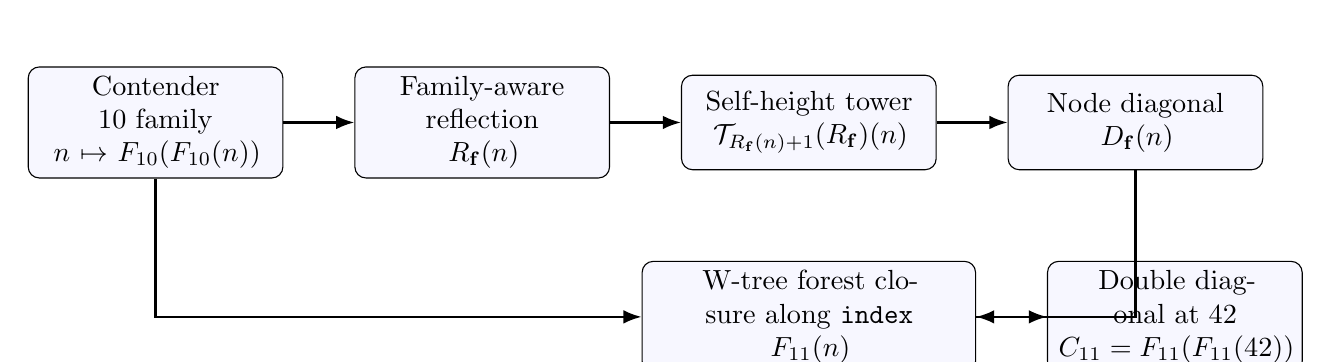
\begin{tikzpicture}[
  box/.style={draw,rounded corners,fill=blue!3,align=center,
              minimum height=1.2cm,text width=3.0cm},
  arr/.style={-{Latex[length=2.3mm]},thick},
  node distance=1.1cm and 0.9cm
]
\node[box] (seed) {Contender 10 family\\$n\mapsto F_{10}(F_{10}(n))$};
\node[box,right=of seed] (family) {Family-aware reflection\\$\Rfam(n)$};
\node[box,right=of family] (tower) {Self-height tower\\$\mathcal T_{\Rfam(n)+1}(\Rfam)(n)$};
\node[box,right=of tower] (diag) {Node diagonal\\$\Dfam(n)$};
\node[box,below=1.15cm of tower,text width=4.0cm] (forest) {W-tree forest closure along \code{index}\\$F_{11}(n)$};
\node[box,right=of forest,text width=3.0cm] (final) {Double diagonal at 42\\$\Celeven=F_{11}(F_{11}(42))$};
\draw[arr] (seed) -- (family);
\draw[arr] (family) -- (tower);
\draw[arr] (tower) -- (diag);
\draw[arr] (diag) |- (forest);
\draw[arr] (seed) |- (forest);
\draw[arr] (forest) -- (final);
\end{tikzpicture}
\caption{Construction pipeline. The tower height is itself the direct
reflection value, and the entire node operator is then iterated along the
self-indexing W-tree.}
\label{fig:pipeline}
\end{figure}

%======================================================================
\section{Formal comparison}
\label{sec:formal}

This section gives the complete mathematical proof architecture mirrored by
\code{Comparison11.lean}. The central point is that every nontrivial semantic
quantity appears beneath an explicit maximum.

\subsection{Direct reflection bounds}

\begin{lemma}[Visible children]
\label{lem:childR}
For every family $\mathbf f$, input $n$, and index $i\le n$,
\[
  \mathbf f(i,n)<\Rfam(n).
\]
\end{lemma}

\begin{proof}
By definition $\mathbf f(i,n)\le P_{\mathbf f}(n)$, and
$P_{\mathbf f}(n)$ is one argument of the maximum in
\cref{eq:reflect11}. The leading $n+1$ turns the resulting weak bound into a
strict one.
\end{proof}

\begin{lemma}[Bounded programs]
\label{lem:programR}
If $t\in\operatorname{CTm}_{\le n}$, then
\[
  \operatorname{Val}_{\widehat{\mathbf f},n}(t)<\Rfam(n).
\]
\end{lemma}

\begin{proof}
The value is at most $M_{\mathbf f}(n)$ by the finite-maximum lemma already
used throughout the repository, and $M_{\mathbf f}(n)$ is the second argument
of the maximum in \cref{eq:reflect11}.
\end{proof}

\begin{lemma}[Input]
\label{lem:inputR}
For all $\mathbf f,n$, $n<\Rfam(n)$.
\end{lemma}

\begin{proof}
Immediate from the additive $n+1$ in \cref{eq:reflect11}.
\end{proof}

In Lean these are \code{oracle\_lt\_reflect11},
\code{fvalue\_lt\_reflect11}, and \code{input\_lt\_reflect11}.

\subsection{Strict growth of the tower}

\begin{lemma}[One more reflection]
\label{lem:towerstep}
For every unary $g$ and every $k,n$,
\[
  \mathcal T_k(g)(n)<\mathcal T_{k+1}(g)(n).
\]
\end{lemma}

\begin{proof}
Unfold one step of the tower. The goal becomes
\[
  \mathcal T_k(g)(n)
  < \code{Fk.reflectFk}(\mathcal T_k(g),n),
\]
which is exactly the incumbent theorem
\code{Fk.oracle\_lt\_reflectFk}.
\end{proof}

\begin{proposition}[Strict monotonicity in tower height]
\label{prop:towermono}
For fixed $g,n$, the function $k\mapsto\mathcal T_k(g)(n)$ is strictly
increasing.
\end{proposition}

\begin{proof}
Induct on the upper height. If $a<b+1$, either $a=b$, in which case
\cref{lem:towerstep} applies directly, or $a<b$, in which case combine the
induction hypothesis with the final step from height $b$ to $b+1$.
\end{proof}

\subsection{What the node diagonal dominates}

\begin{theorem}[Self-height tower closure]
\label{thm:towerclosure}
For every family $\mathbf f$, input $n$, and height $k\le\Rfam(n)$,
\[
  \mathcal T_k(\Rfam)(n)<\Dfam(n).
\]
\end{theorem}

\begin{proof}
The hypothesis gives $k<\Rfam(n)+1$. By
\cref{prop:towermono},
\[
  \mathcal T_k(\Rfam)(n)
  <\mathcal T_{\Rfam(n)+1}(\Rfam)(n).
\]
The latter is an explicit argument of the maximum in
\cref{eq:diagonal11}, hence is strictly below $\Dfam(n)$.
\end{proof}

\begin{corollary}[Input-bounded towers]
If $k\le n$, then
\[
  \mathcal T_k(\Rfam)(n)<\Dfam(n).
\]
\end{corollary}

\begin{proof}
By \cref{lem:inputR}, $n<\Rfam(n)$, so $k\le\Rfam(n)$ and
\cref{thm:towerclosure} applies.
\end{proof}

The direct reflection itself is another explicit argument of the maximum, so
$\Rfam(n)<\Dfam(n)$. Combining this with
\cref{lem:childR,lem:programR,lem:inputR} gives:

\begin{theorem}[Node domination]
\label{thm:nodedom}
At every node and input~$n$, $\Dfam(n)$ strictly exceeds:
\begin{enumerate}[leftmargin=*]
\item the input~$n$;
\item every visible child $\mathbf f(i,n)$ with $i\le n$;
\item every accepted kind-polymorphic program in the depth-$n$ enumeration,
  relative to the packed child family; and
\item every unary reflection tower over $\Rfam$ of height at most $\Rfam(n)$.
\end{enumerate}
\end{theorem}

\subsection{Forest edges}

\begin{lemma}[Strict child edge]
\label{lem:forestedge}
Let $g:\N\to W$ be the children of a tree node. For every $i\le n$,
\[
  S(\mathbf s,g(i))(n)
  < S(\mathbf s,\operatorname{node}(g))(n).
\]
\end{lemma}

\begin{proof}
At the parent, the oracle family is
$\mathbf f_g(j,m)=S(\mathbf s,g(j))(m)$. Apply the visible-child part of
\cref{thm:nodedom} with index~$i$.
\end{proof}

The Lean theorem is \code{stage11\_child\_lt}. The companion theorem
\code{input\_lt\_stage11} follows by cases on the tree and the input part of
\cref{thm:nodedom}.

\subsection{The seed path inside the self-index}

The proof that $F_{11}$ dominates its seed uses a fixed three-edge path already
present in the repository's comparison for Contender~9. The tree
\code{index} is a node whose child~0 is \code{treesOfDepth 0}. That tree is a
node whose child~0 is the tree denoted by the first depth-0 term; the repository
proves that this tree is \code{leaf}. Hence, at every input~$n$,
\begin{align*}
\operatorname{family10}(n)
&<S(\operatorname{const}(\operatorname{family10}),\operatorname{leaf})(n)\\
&<S(\operatorname{const}(\operatorname{family10}),\code{treesOfDepth 0})(n)\\
&<S(\operatorname{const}(\operatorname{family10}),\code{index})(n)\\
&=F_{11}(n).
\end{align*}
The first inequality is node domination of the seed value; the next two are
instances of \cref{lem:forestedge} with child index~0. This is formalized as
\code{family10\_lt\_F11}.

\subsection{The central theorem}

\begin{theorem}[Contender 11 beats Contender 10]
\label{thm:main}
\[
  \Cten<\Celeven.
\]
Equivalently, the Lean target is
\[
  \code{contender\_10 < contender\_11}.
\]
\end{theorem}

\begin{proof}
By definitional equality,
$\Cten=\operatorname{family10}(42)$. The seed-path theorem gives
\[
  \Cten<F_{11}(42).
\]
The input theorem for the stage at input $F_{11}(42)$ gives
\[
  F_{11}(42)<F_{11}(F_{11}(42))=\Celeven.
\]
Transitivity completes the proof.
\end{proof}

The corresponding Lean proof is deliberately short:

\begin{lstlisting}
theorem contender_10_lt_contender_11 :
    contender_10 < contender_11 :=
  Nat.lt_trans (family10_lt_F11 42)
    (input_lt_stage11
      (fun _ => family10) index (F11 42))
\end{lstlisting}

\subsection{Domination of W-definable trees}

The same enumeration argument used for earlier forest contenders lifts
unchanged.

\begin{theorem}[Eventual domination of every represented tree]
\label{thm:eventual}
If a W-language term $t$ occurs in the finite enumeration at depth~$k$, then
there exists $N$ such that for every $n\ge N$,
\[
  S(\operatorname{const}(\operatorname{family10}),
    \operatorname{defTree}(t))(n)
  <F_{11}(n).
\]
\end{theorem}

\begin{proof}
Choose the enumeration position~$i$ of~$t$ and take $N=k+i$. At any
$n\ge N$, both $i\le n$ and $k\le n$. The represented tree is therefore a
visible child of \code{treesOfDepth k}, and that depth tree is a visible child
of \code{index}. Apply \cref{lem:forestedge} twice.
\end{proof}

The theorem appears as \code{defined\_tree\_eventually\_lt11}.

%======================================================================
\section{Why the increase is substantial}

The only unconditional numerical claim needed for acceptance is
\cref{thm:main}. Nevertheless, the construction supplies a much richer margin
than ``predecessor plus one.'' Four independent facts support that assessment.

\subsection{It closes the incumbent reflection under self-height iteration}

Contender~10 applies \code{Fk.reflectFk} to the Contender~9 family and then uses
an outer double application. At a Contender~11 node, the direct family-aware
reflection value $\Rfam(n)$ is itself used as the height of a new tower of
\code{Fk.reflectFk} applications. This is not a fixed iterate chosen in the
source, and not merely $n$ iterations. The height is already larger than the
input, every visible child, and every bounded accepted program value.

The formal theorem \cref{thm:towerclosure} is therefore a useful intermediate
result in its own right: one node of the new construction dominates every
reflection tower whose height is at most the direct reflection value at that
node.

\subsection{The reflection sees an entire child family}

A unary tower alone would amplify only one seed function. Here the direct seed
at each node is a reflection relative to the packed family of all child
stages. Programs in the object language may decode a dynamically computed
child index and argument. Independently, the explicit prefix maximum makes the
basic child inequality immune to whether a suitable selector program appears
in the bounded enumeration.

This two-channel access is deliberate:
\begin{itemize}[leftmargin=*]
\item \emph{semantic access}: programs can combine and iterate child stages in
  ways determined at run time;
\item \emph{comparison access}: the proof can point directly to a finite prefix
  maximum and does not need to synthesize a selector program.
\end{itemize}

\subsection{The node operator is iterated along internal trees}

The self-height tower is not applied once at the root. It is the local
operation at every node of \code{index}. The index is not a hand-written
finite ordinal notation. Its branches range over all W-trees denoted by the
repository's W-language, grouped by syntax depth. Thus the same strong local
closure is propagated through an internally generated family of well-founded
shapes.

\subsection{The final double application remains}

After building the forest-closed family $F_{11}$, the final number uses the
same robust double diagonal pattern as Contenders~7--10:
\[
  F_{11}(F_{11}(42)).
\]
The first value is already larger than \Cten; the second call uses that value
as the syntax budget, program-checker fuel, prefix length, tower input, and
forest visibility bound throughout the construction.

%======================================================================
\section{Computability and constructive legitimacy}

\subsection{Why the number is computable in principle}

Every operation in the definition is total:

\begin{enumerate}[leftmargin=*]
\item \code{Fk.ctmsUpTo n} is a structurally recursive finite list.
\item \code{Fk.fvalue} uses a decidable bounded type checker and the existing
  total normalizer. The normalizer's termination argument is supplied by the
  formal strong-normalization development for the object language.
\item \code{BigNumber.maximum} and \code{W.prefixMax} traverse finite lists or
  finite prefixes.
\item \code{towerFk k f} is primitive recursion on the natural number~$k$.
\item \code{stage11} is structural recursion on a well-founded W-tree, in the
  same form already accepted for earlier contenders.
\item \code{F11} and \code{contender\_11} are ordinary compositions of these
  total functions.
\end{enumerate}

There is no search for a halting witness, no maximum over all programs without
a finite syntax bound, and no appeal to an uncomputable oracle. Given unlimited
resources, reduction of \code{contender\_11} reaches a numeral.

\subsection{Why one should never try to evaluate it}

Computable does not mean feasible. Even at modest inputs the syntax lists grow
combinatorially, accepted terms can have enormous normal forms, and each
reflection level embeds a maximum over all values from the preceding oracle.
The self-height tower asks for a number of reflection layers equal to an
already enormous reflected value. The W-tree closure then repeats that node
operator recursively.

The repository's standard instruction therefore applies with extra force:
check the definitions and proofs, but do not evaluate the contender. Kernel
checking manipulates the compact syntax and proof terms; evaluation would try
to realize the represented natural number.

\subsection{Axioms and proof irrelevance}

The new definitions add no axioms. They inherit the same metatheoretic
foundation as Contender~10. The supplied audit prints the axiom dependencies of
the new number and major comparison theorems and accepts only
\code{propext} and \code{Quot.sound}, matching the repository policy. The audit
also traverses the declaration closure of \code{contender\_11} and rejects any
occurrence of the closed constants \code{contender\_10} through
\code{contender\_5}.

%======================================================================
\section{Proof-theoretic interpretation: heuristic only}

The formal proof above deliberately avoids assigning an ordinal to the
kind-polymorphic language or to the combined closure. That restraint is
important. Exact proof-theoretic calibration of impredicative polymorphic
systems, especially after oracle relativization and interaction with
self-indexing W-trees, is subtle. A persuasive fast-growing-hierarchy slogan is
not a substitute for a theorem.

Still, the construction has a clear qualitative reading. Let $\alpha$ denote,
only schematically, the strength associated with one kind-polymorphic
reflection step over a fixed oracle. Then:

\begin{itemize}[leftmargin=*]
\item one application of \code{reflectFk} behaves like one strong reflection
  increment over the oracle;
\item a tower of height~$k$ iterates that increment $k$ times;
\item choosing $k=\Rfam(n)+1$ diagonalizes the iteration length against a
  value already produced by the reflected system; and
\item forest closure repeats this diagonal operation along W-language-definable
  well-founded trees.
\end{itemize}

This suggests a jump far beyond a fixed finite stack of Contender~10-style
reflections. The archive does \emph{not} claim an exact ordinal identity, a
complete domination theorem over all functions definable in some external
foundational theory, or a separation result between proof-theoretic systems.
Those would require a separate metamathematical development.

The strongest rigorous growth statement currently supplied is internal and
finite: \cref{thm:towerclosure}, together with forest child domination and
\cref{thm:eventual}. These are already enough to show that the proposal is not
merely a constant-size arithmetic wrapper.

%======================================================================
\section{Lean artifact architecture}

\subsection{Definition module}

\code{BusyLean/Contender11.lean} contains only the definitions required to name
the number:

\begin{longtable}{>{\ttfamily}p{0.28\textwidth} p{0.64\textwidth}}
\toprule
\normalfont Declaration & Purpose \\
\midrule
\endfirsthead
\toprule
\normalfont Declaration & Purpose \\
\midrule
\endhead
reflect11 & Family-aware bounded kind-polymorphic reflection. \\
towerFk & Finite iteration of the existing unary reflection operator. \\
diagonal11 & Maximum of the direct reflection and its self-height tower, plus the input guard. \\
stage11 & W-tree recursion placing the diagonal at every node. \\
family10 & Contender~10's construction viewed as an input family. \\
F11 & Forest closure along \code{index}. \\
contender\_11 & The final closed natural $F_{11}(F_{11}(42))$. \\
\bottomrule
\end{longtable}

Keeping comparisons out of the definition module is consistent with the
repository's timed build discipline: the definition phase can be measured
separately from theorem elaboration.

\subsection{Comparison module}

\code{BusyLean/Comparison11.lean} is organized in four layers:

\begin{enumerate}[leftmargin=*]
\item arithmetic bounds for \code{reflect11};
\item strict monotonicity of \code{towerFk};
\item node and forest domination theorems; and
\item seed, contender, and definable-tree comparisons.
\end{enumerate}

The proof intentionally reuses the public comparison interface of Contender~10,
not the internal normalization proof. In particular,
\code{towerFk\_step\_lt} is one line after unfolding because
\code{Fk.oracle\_lt\_reflectFk} already states exactly the needed inequality.

\subsection{Audit and replay}

\code{test/Audit11.lean} contains:
\begin{itemize}[leftmargin=*]
\item \code{\#print axioms} commands for the number and major theorems;
\item a transitive declaration-closure command that rejects all prior closed
  contender constants; and
\item \code{\#check} commands recording the central signatures.
\end{itemize}

\code{scripts/check\_contender11.py} performs the repository-style clean build,
enforces time budgets, runs the audit, parses its output, and rejects forbidden
axioms. The patch also adds the two modules to \code{BusyLean.lean}.

%======================================================================
\section{Reproducibility and verification status}

\subsection{Applying the proposal}

Starting from the pinned commit, the intended replay is:

\begin{lstlisting}[language={}]
git checkout 4c4b03d0e2003c479e3bee90a21c8bea13f66c40
git apply patches/contender11.patch
python3 scripts/check_contender11.py
\end{lstlisting}

Equivalently, copy the files from the archive's \code{lean/} directory into the
matching repository paths and add the two imports to \code{BusyLean.lean}.

\subsection{Validation completed in this artifact build}

The following checks were run while producing the archive:

\begin{enumerate}[leftmargin=*]
\item the LaTeX article was compiled to PDF;
\item the PDF was rendered page by page and visually inspected for clipping,
  overlap, black boxes, and broken glyphs;
\item the Python replay script was syntax-checked;
\item a static policy scanner checked the new definition for forbidden Lean
  features and checked that executable code does not reference a prior closed
  contender constant;
\item the integration patch was applied with \code{git apply --check} to a
  reconstructed pinned-file skeleton; and
\item SHA-256 hashes were generated for the deliverables.
\end{enumerate}

\begin{status}
A Lean~4.34.0 executable was not available in the artifact-building container,
and the official binary could not be materialized through the available file
transport. Therefore this report does not claim that the new modules were
kernel-replayed here. The proof scripts were reviewed against the pinned source
interfaces and are accompanied by an exact replay command. Repository
acceptance should be conditional on a successful run of
\code{python3 scripts/check\_contender11.py} in the pinned checkout.
\end{status}

This limitation affects confidence in elaboration details, not the mathematical
comparison argument: the latter is given explicitly in \cref{sec:formal} and
uses only the stated incumbent lemmas. Possible replay failures would most
likely be local syntactic or inference issues and should not require changing
the construction.

\subsection{Expected audit outcome}

A successful replay should establish all of the following:

\begin{itemize}[leftmargin=*]
\item the definition module elaborates within the 15-second budget;
\item the comparison module and complete library elaborate within the
  60-second proof budget;
\item no axiom outside \code{propext} and \code{Quot.sound} appears in the
  audited declarations;
\item \code{contender\_11}'s declaration closure avoids
  \code{contender\_10}, \code{contender\_9}, and all earlier contender
  constants; and
\item the theorem \code{contender\_10\_lt\_contender\_11} is accepted by the
  Lean kernel.
\end{itemize}

%======================================================================
\section{Risk analysis}

\subsection{Formalization risks}

The proposal is intentionally conservative in its use of new Lean machinery.
The main residual risks are:

\begin{enumerate}[leftmargin=*]
\item \textbf{Elaboration of the function-valued recursion.} The return type of
  \code{towerFk} is curried. This is standard structural recursion, but the
  exact equation reduction should be confirmed on Lean~4.34.0.
\item \textbf{Strict-monotonicity proof inference.} The induction in
  \code{towerFk\_strictMono} uses only natural arithmetic and the one-step
  theorem. If elaboration is sensitive, it can be replaced by an explicitly
  quantified two-height lemma without changing any definition.
\item \textbf{Timing.} The new definition is syntactically small and reuses
  precompiled Contender~10 modules, so it is expected to fit comfortably.
  Only an actual clean build can certify the repository's machine-relative
  timing rule.
\item \textbf{Axiom reporting through inherited normalization proofs.} The new
  number inherits the same proof-carrying normalizer as Contender~10. The audit
  is included precisely to ensure the inherited closure stays within the
  repository's allowed pair of axioms.
\end{enumerate}

None of these risks concerns termination of the mathematical construction or
validity of the inequality argument.

\subsection{Metamathematical risks}

No exact proof-theoretic ordinal is claimed. A future calibration could reveal
that some apparently different amplification mechanisms collapse under an
appropriate equivalence. Such a result would not invalidate the strict
numerical theorem or the internal tower-domination theorems. It would only
refine the informal account of how large the margin is.

%======================================================================
\section{Further research questions}

The construction suggests several concrete next projects.

\begin{enumerate}[leftmargin=*]
\item \textbf{Kernel replay and proof minimization.} Run the pinned audit,
  remove any unnecessary uses of \code{omega}, and seek an axiom-free arithmetic
  comparison layer if the inherited definitions permit it.
\item \textbf{Uniform tower domination.} Strengthen
  \code{fixedTower\_lt\_diagonal11} from a pointwise height bound to domination
  of a class of height functions $h(n)\le\Rfam(n)$, with a reusable Lean API.
\item \textbf{Internal tower coding.} Construct explicit kind-polymorphic terms
  that realize selected reflection-tower patterns, clarifying how much of the
  external tower can be represented inside the object language.
\item \textbf{Self-index from the stronger language.} The current tree index is
  inherited from the W-language because it has a direct Lean set-theoretic
  interpretation. Develop a safe syntax of well-founded codes generated by the
  kind-polymorphic language itself, together with a total decoding theorem.
\item \textbf{Predicative kind-universe ladder.} Implement a stratified sequence
  of kind universes and diagonalize over the number of levels, as anticipated
  in the repository roadmap. Compare that language-level jump with the present
  external self-height closure.
\item \textbf{Large elimination.} Build a realizability model for a carefully
  chosen dependently typed object language with natural-number elimination into
  types, retaining a total executable normalizer and a sound bounded checker.
\item \textbf{Formal growth separations.} Identify restricted fragments for
  which one can prove that a self-height tower eventually dominates every fixed
  tower, rather than relying only on the pointwise theorem supplied here.
\item \textbf{Resource-certified checking.} Extend the audit so that the timing
  report, toolchain hash, source commit, and axiom output are emitted as a
  machine-readable attestation committed with each contender.
\item \textbf{Alternative diagonal heights.} Compare $\Rfam(n)+1$ with heights
  such as $\Dfam(n)$ truncated through a structurally decreasing recursion,
  or heights generated by a separate W-recursive rank, while preserving obvious
  totality and simple comparison proofs.
\item \textbf{Proof-theoretic calibration.} Develop a rigorous ordinal or
  reflection-theoretic analysis of kind-polymorphic $F_\omega$ with oracles,
  then analyze finite iteration and W-tree closure as separate operations.
\end{enumerate}

%======================================================================
\section{Conclusion}

Contender~11 is a conservative formal extension and an aggressive growth
extension. It does not add a new evaluator, axiom, or unbounded search. Instead,
it composes three mechanisms already justified in \repo{}:

\begin{enumerate}[leftmargin=*]
\item kind-polymorphic reflection over a total object language;
\item computable packing of an oracle family; and
\item forest reflection along a self-indexing W-tree.
\end{enumerate}

The new contribution is the self-height diagonal between the first and third
mechanisms. At each node, the result of direct family-aware reflection chooses
the height of an entire subsequent reflection tower. Explicit maxima make the
key theorem elementary, while the recursive placement of that diagonal along
\code{index} supplies a substantial structural margin.

The resulting closed natural
\[
  \boxed{\Celeven=F_{11}(F_{11}(42))}
\]
is computable in principle and is accompanied by a short formal comparison
script, an axiom/dependency audit, a timed replay script, an integration patch,
and this detailed argument. The remaining acceptance step is mechanical but
essential: replay the archive under Lean~4.34.0 at the pinned repository commit.

%======================================================================
\appendix
\section{Principal Lean definitions}

For review convenience, the core definition module is reproduced below in a
compact form. The authoritative source is
\code{lean/BusyLean/Contender11.lean} in the archive.

\begin{lstlisting}
import BusyLean.Contender10

namespace BusyLean

def reflect11 (fs : W.Family) (n : Nat) : Nat :=
  n + 1 + BigNumber.maxN
    (W.prefixMax (fun i => fs i n) n)
    (BigNumber.maximum
      (Fk.fvalue (packFamily fs) n)
      (Fk.ctmsUpTo n))

def towerFk : Nat -> (Nat -> Nat) -> Nat -> Nat
  | 0, f     => f
  | Nat.succ k, f => Fk.reflectFk (towerFk k f)

def diagonal11 (fs : W.Family) (n : Nat) : Nat :=
  n + 1 + BigNumber.maxN
    (reflect11 fs n)
    (towerFk (reflect11 fs n + 1)
      (reflect11 fs) n)

def stage11 (seed : W.Family) :
    BigNumber.WTree Nat -> Nat -> Nat
  | .leaf   => diagonal11 seed
  | .node g => diagonal11
      (fun i => stage11 seed (g i))

def family10 (n : Nat) : Nat := F10 (F10 n)

def F11 (n : Nat) : Nat :=
  stage11 (fun _ => family10) index n

def contender_11 : Nat := F11 (F11 42)

end BusyLean
\end{lstlisting}

\section{Principal theorem signatures}

\begin{lstlisting}
theorem oracle_lt_reflect11
  (fs : W.Family) {i n : Nat} (hi : i <= n) :
  fs i n < reflect11 fs n

theorem fvalue_lt_reflect11
  (fs : W.Family) {n : Nat} {t : Fk.CTm}
  (ht : t in Fk.ctmsUpTo n) :
  Fk.fvalue (packFamily fs) n t < reflect11 fs n

theorem towerFk_step_lt
  (f : Nat -> Nat) (k n : Nat) :
  towerFk k f n < towerFk (k + 1) f n

theorem fixedTower_lt_diagonal11
  (fs : W.Family) {k n : Nat}
  (hk : k <= reflect11 fs n) :
  towerFk k (reflect11 fs) n < diagonal11 fs n

theorem stage11_child_lt
  (seed : W.Family)
  (g : Nat -> BigNumber.WTree Nat)
  {i n : Nat} (hi : i <= n) :
  stage11 seed (g i) n < stage11 seed (.node g) n

theorem family10_lt_F11 (n : Nat) :
  family10 n < F11 n

theorem contender_10_lt_contender_11 :
  contender_10 < contender_11
\end{lstlisting}

The actual source uses Lean's membership symbol in two signatures; the ASCII
word \code{in} above is expository pseudocode, not a replacement for the
archive's authoritative module.

\section{Artifact inventory}

\begin{longtable}{>{\ttfamily}p{0.43\textwidth} p{0.49\textwidth}}
\toprule
\normalfont Path & Purpose \\
\midrule
\endfirsthead
\toprule
\normalfont Path & Purpose \\
\midrule
\endhead
article/contender11.tex & This paper's LaTeX source. \\
article/contender11.pdf & Compiled and rendered paper. \\
lean/BusyLean/Contender11.lean & New closed-number definitions. \\
lean/BusyLean/Comparison11.lean & Strict comparison and structural domination theorems. \\
lean/test/Audit11.lean & Axiom and dependency closure audit. \\
lean/scripts/check\_contender11.py & Clean-build, timing, and audit driver. \\
patches/contender11.patch & Patch against the pinned BusyLean commit. \\
notes/FORMAL\_CLAIMS.md & Claim-by-claim map from mathematics to declarations. \\
notes/REPRODUCE.md & Exact integration and replay instructions. \\
validation/static\_validation.txt & Results of artifact-level static checks. \\
validation/pdf\_inspection.txt & PDF render and visual inspection record. \\
MANIFEST.sha256 & SHA-256 inventory of final files. \\
\bottomrule
\end{longtable}

\begin{thebibliography}{9}
\bibitem{BusyLean}
V.~Reshetnikov and contributors,
\emph{BusyLean: name the biggest number, in Lean},
GitHub repository, commit
\commitid, 2026.

\bibitem{GirardF}
J.-Y.~Girard,
\emph{Interpr\'etation fonctionnelle et \'elimination des coupures de
l'arithm\'etique d'ordre sup\'erieur},
Th\`ese d'\'Etat, Universit\'e Paris VII, 1972.

\bibitem{Reynolds}
J.~C.~Reynolds,
Towards a theory of type structure,
in \emph{Programming Symposium}, Lecture Notes in Computer Science 19,
Springer, 1974, pp.~408--425.

\bibitem{CoquandHuet}
T.~Coquand and G.~Huet,
The calculus of constructions,
\emph{Information and Computation} 76 (1988), 95--120.

\bibitem{Howard}
W.~A.~Howard,
Ordinal analysis of terms of finite type,
\emph{Journal of Symbolic Logic} 45 (1980), 493--504.
\end{thebibliography}

\end{document}
